\chapter{Analytic \texorpdfstring{\(L\)}{L}-functions}
  Throughout, \(s = \s+it\) and \(u = \tau+ir\) will stand for complex variables with \(\s\), \(\tau\), \(t\), and \(r\) real. We also write
  \[
    (u)_{k} = u(u+1) \cdots (u+(k-1)),
  \]
  for the Pochhammer symbol. We will also make use of various properties of the gamma function developed in \cref{sec:the_gamma_function}. Also, all sums and products over zeros of a complex function will be counted with multiplicity and ordered with respect to the size of the ordinate.
  \section{Analytic Data}
    An \textbf{analytic \(L\)-function}\index{analytic \(L\)-function} \(L(s)\) is a Dirichlet series
    \[
      L(s) = \sum_{n \ge 1}\frac{a_{L}(n)}{n^{s}},
    \]
    with coefficients \(a_{L}(n) \in \C\) such that \(a_{L}(1) = 1\) and satisfying the following properties:
    \begin{enumerate}[align=left]
      \item[\textbf{Analyticity:}] There exists a nonnegative integer \(m_{L}\) such that the Dirichlet series of \(L(s)\) is absolutely convergent for \(\s > 1\) and admits meromorphic continuation to \(\C\) with at most a pole at \(s = 1\) of order \(m_{L}\). Moreover, \((s-1)^{m_{L}}L(s)\) is order \(1\).
      \item[\textbf{Functional Equation:}] There is a positive integer \(q_{L}\), called the \textbf{conductor}\index{conductor} of \(L(s)\), a positive integer \(d_{L}\) called the \textbf{degree}\index{degree} of \(L(s)\), complex numbers \((\mu_{j})_{j \le d_{L}}\) called the \textbf{gamma parameters}\index{gamma parameters} of \(L(s)\) that are either real or occur in conjugate pairs and satisfy \(\Re(\mu_{j}) \ge 0\), and a complex number \(\e_{L}\) called the \textbf{root number}\index{root number} of \(L(s)\) with \(|\e_{L}| = 1\), all of which determine functions
      \[
        \g(s,L) = \pi^{-\frac{d_{L}s}{2}}\prod_{j}\G\left(\frac{s+\mu_{j}}{2}\right) \quad \text{and} \quad \L(s,L) = q_{L}^{\frac{s}{2}}\g(s,L)L(s),
      \]
      called the \textbf{gamma factor}\index{gamma factor} of \(L(s)\) and the \textbf{completion}\index{completion} of \(L(s)\) respectively, where the latter satisfies
      \[
        \L(s,L) = \e_{L}\conj{\L(1-\conj{s},L)}.
      \]
      This is called the \textbf{functional equation}\index{functional equation} for \(L(s)\). The tuple \((\e_{L},q_{L},\mu_{1},\ldots,\mu_{d_{L}})\) is called the \textbf{functional equation data}\index{functional equation data} of \(L(s)\).
      \item[\textbf{Euler product:}] For every prime \(p\), there exist complex numbers \((\a_{j}(p))_{j \le d_{L}}\) called the \textbf{Euler parameters}\index{Euler parameters} of \(L(s)\) at \(p\) satisfying \(|\a_{j}(p)| \le p^{\t_{L}}\) for some \(0 \le \t_{L} < 1\) and are such that \(L(s)\) admits the Euler product
      \[
        L(s) = \prod_{p}(1-\a_{1}(p)p^{-s})^{-1} \cdots (1-\a_{d_{L}}(p)p^{-s})^{-1},
      \]
      for \(\s > 1\). The polynomial \(L_{p}\) defined by
      \[
        L_{p}(T) = (1-\a_{1}(p)T) \cdots (1-\a_{d_{L}}(p)T),
      \]
      is called the \textbf{Euler factor}\index{Euler factor} of \(L(s)\) at \(p\). If \(p \nmid q_{L}\) then \(L_{p}\) is of degree \(d_{L}\) while if \(p \mid q_{L}\) then \(L_{p}\) is of degree less than \(d_{L}\). In the former case we say \(p\) is \textbf{unramified}\index{unramified} while in the latter we say \(p\) is \textbf{ramified}\index{ramified}.
    \end{enumerate}

    An analytic \(L\)-function is said to be \textbf{Selberg class}\index{Selberg class} if it satisfies the following additional property:

    \begin{enumerate}[align=left]
      \item[\textbf{Ramanujan bound:}] We may take \(\t_{L} = 0\) so that \(|\a_{j}(p)| \le 1\).
    \end{enumerate}

    Some comments on the definition of analytic \(L\)-functions are in order.
    \begin{enumerate}[label*=(\roman*)]
      \item As the Dirichlet series of \(L(s)\) converges absolutely for \(\s > 1\) its converges locally absolutely uniformly in this half-plane and therefore defines a holomorphic function there. Moreover, the Euler product necessarily converges locally absolutely uniformly in the same half-plane and hence defines a holomorphic function there as well which agrees with the Dirichlet series.
      \item The bound \(\Re(\mu_{j}) \ge 0\) ensures that the gamma factor is holomorphic in the half-plane \(\s > 0\). As this factor is then guaranteed to be finite and nonzero at \(s = 1\), the completion possesses a pole at \(s = 1\) of order \(r\). By the functional equation, the completion also has a pole at \(s = 0\) of the same order.
      \item If we merely assume \((s-1)^{m_{L}}L(s)\) is finite order then the functional equation forces the order to be \(1\). This can be deduced by considering the entire function
      \[
        s^{m_{L}}(s-1)^{m_{L}}\L(s,L),
      \]
      and applying the Phragm\'en-Lindel\"of convexity principle in vertical strips.
      \item The condition that the root number satisfies \(|\e_{L}| = 1\) isn't strictly necessary. For applying the functional equation twice shows \(|\e_{L}|^{2} = 1\).
      \item As the gamma function is conjugation-equivariant and the gamma parameters are real or occur in conjugate pairs, the gamma factor is also conjugation-equivariant. This means that we can write the functional equation in the form
      \[
        q_{L}^{\frac{s}{2}}\g(s,L)L(s) = \e_{L}q_{L}^{\frac{1-s}{2}}\g(1-s,L)\conj{L(1-\conj{s})}.
      \]
      \item The Euler product implies that the coefficients \(a_{L}(n)\) are multiplicative and are determined on prime powers by
      \[
        a_{L}(p^{k}) = \sum_{j_{1} \le \cdots \le j_{k}}\a_{j_{1}}(p) \cdots \a_{j_{k}}(p).
      \]
      In other words, \(a_{L}(p^{k})\) is the complete symmetric polynomial of degree \(k\) in the Euler parameters at \(p\). If the Ramanujan bound holds, then it follows that \(a_{L}(n) \ll \s_{d_{L}}(n)\). This implies the slightly weaker, but more practical, estimate \(a_{L}(n) \ll_{\e} n^{\e}\).
    \end{enumerate}

    We will also define the \textbf{dual}\index{dual} \(\conj{L}(s)\) of \(L(s)\) by
    \[
      \conj{L}(s) = \conj{L(\conj{s})}.
    \]
    Analytic \(L\)-functions are closed under duals. Indeed, \(\conj{L}(s)\) is an analytic \(L\)-function with coefficients \(a_{\conj{L}}(n) = \conj{a_{L}(n)}\), a pole at \(s = 1\) of order \(m_{\conj{L}} = m_{L}\), conductor \(q_{\conj{L}} = q_{L}\), degree \(d_{\conj{L}} = d_{L}\), gamma parameters \((\conj{\mu_{j}})_{j \le d_{L}}\), root number \(\e_{\conj{L}} = \conj{\e_{L}}\), gamma factor \(\g(s,\conj{L}) = \g(s,L)\), completion \(\L(s,\conj{L}) = \conj{\L(\conj{s},L)}\), and Euler parameters \((\conj{\a_{j}(p)})_{j \le d_{L}}\) at \(p\). Moreover, the dual of \(L(s)\) is Selberg class if \(L(s)\) is. We also say \(L(s)\) is \textbf{self-dual}\index{self-dual} if it is equal to its dual. This is equivalent to the coefficients \(a_{L}(n)\) being real. In any case, we can express the functional equation as
    \[
      \L(s,L) = \e_{L}\L(1-s,\conj{L}),
    \]
    so the functional equation relates an analytic \(L\)-function with its dual. This formula will also be useful when taking derivatives of the functional equation.

    It is clear from the definition that analytic \(L\)-functions are closed under multiplication and that the degree is additive. Moreover, this closure respects Selberg class \(L\)-functions. This makes the set of analytic \(L\)-functions into a graded commutative semigroup where the grading is induced by degree. It follows that there exist irreducible elements with respect to the grading and we say that an analytic \(L\)-function is \textbf{primitive}\index{primitive} if it such an irreducible. Clearly any analytic \(L\)-function of degree \(1\) is primitive. Moreover, every analytic \(L\)-function factors into a product of primitive \(L\)-functions. Such a factorization is only conjectured to be unique for Selberg class \(L\)-functions. A sufficient condition would be \textbf{Selberg's orthogonality conjecture}\index{Selberg's orthogonality conjecture}.

    \begin{conjecture*}[Selberg's orthogonality conjecture]
      For any two primitive Selberg class \(L\)-functions \(L_{1}(s)\) and \(L_{2}(s)\), we have
      \[
        \sum_{p \le x}\frac{a_{L_{1}}(p)\conj{a_{L_{2}}(p)}}{p} = \d_{L_{1},L_{2}}\log\log(x)+O(1).
      \]
    \end{conjecture*}

    Indeed, we have the following result:

    \begin{proposition}
      Assume Selberg's orthogonality conjecture. Then every Selberg class \(L\)-function factors uniquely into a product of primitive Selberg class \(L\)-functions.
    \end{proposition}
    \begin{proof}
      If the factorization into primitive unity \(L\)-functions were not unique, then we would have distinct factorizations satisfying
      \[
        L_{1}(s) \cdots L_{n}(s) = M_{1}(s) \cdots M_{m}(s),
      \]
      for some primitive Selberg class \(L\)-functions \(L_{i}\) and \(M_{j}\). By uniqueness of coefficients of Dirichlet series, compare the \(p\)-th coefficient to see that
      \[
        \sum_{i}a_{L_{i}}(p) = \sum_{j}a_{M_{j}}(p).
      \]
      Now consider
      \[
        \sum_{p < x}\frac{1}{p}\left(\sum_{i}a_{L_{i}}(p)\right)\left(\sum_{j}\conj{a_{M_{j}}(p)}\right) = \sum_{i,j}\sum_{p < x}\frac{a_{L_{i}}(p)\conj{a_{M_{j}}(p)}}{p}.
      \]
      Selberg's orthogonality conjecture implies
      \[
        O(1) = c\log\log(x)+O(1),
      \]
      for some positive integer \(c\) since the factorizations are distinct. This is impossible and thus the factorization is unique.
    \end{proof}

    To an analytic \(L\)-function \(L(s)\), we associate its \textbf{analytic conductor}\index{analytic conductor} \(\mf{q}(s,L)\) defined by
    \[
      \mf{q}(s,L) = q_{L}\mf{q}_{\infty}(s,L),
    \]
    where
    \[
      \mf{q}_{\infty}(s,L) = \prod_{j}(|s+\mu_{j}|+3).
    \]
    For convenience, we will also set
    \[
      \mf{q}(L) = \mf{q}(0,L) \quad \text{and} \quad \mf{q}_{\infty}(L) = \mf{q}_{\infty}(0,L).
    \]
    The choice of \(3\) in \(|s+\mu_{j}|+3\) is a matter of convenience as could use any positive constant. In particular, it is useful when taking logarithms as \(\log(|s+\mu_{j}|+3) \ge 1\). Estimates for the analytic conductor follow from those of the gamma function. Recall from Stirling's formula (see \cref{sec:the_gamma_function}) that
    \begin{equation}\label{equ:vertical_strip_gamma_estimates}
      \G(s) \ll_{\e} (|t|+3)^{\s-\frac{1}{2}}e^{-\frac{\pi}{2}|t|} \quad \text{and} \quad \frac{1}{\G(s)} \ll (|t|+3)^{\frac{1}{2}-\s}e^{\frac{\pi}{2}|t|},
    \end{equation}
    for bounded \(\s\) provided that in the former estimate \(s\) is at least distance \(\e\) away from the poles of the gamma function. Hence
    \[
      \frac{\G(1-s)}{\G(s)} \ll_{\e} (|t|+3)^{1-2\s},
    \]
    for bounded \(\s\) provided \(s\) is at least distance \(\e\) away from the poles of \(\G(1-s)\). Then the estimates
     \begin{equation}\label{equ:gamma_factor_analytic_conductor_estimate}
      \frac{\g(1-s,L)}{\g(s,L)} \ll_{\e} \mf{q}_{\infty}(s,L)^{\frac{1}{2}-\s} \quad \text{and} \quad q_{L}^{\frac{1}{2}-s}\frac{\g(1-s,L)}{\g(s,L)} \ll_{\e} \mf{q}(s,L)^{\frac{1}{2}-\s},
    \end{equation}
    hold for bounded \(\s\) provided \(s\) is at least distance \(\e\) away from the poles of \(\g(1-s,L)\). An associated estimate can be obtain for the logarithmic derivative of the analytic conductor. Recall from the logarithm of Stirling's formula (see \cref{sec:the_gamma_function}) that
    \[
      \frac{\G'}{\G}(s) \ll \log(|s|+3),
    \]
    provided \(\s\) is bounded and \(s\) is at least distance \(\e\) away from the poles of the gamma function. Then the estimates
    \begin{equation}\label{equ:digamma_gamma_factor_analytic_conductor_estimate}
      \frac{\g'}{\g}(s,L) \ll_{\e} \log\mf{q}_{\infty}(s,L) \quad \text{and} \quad \log(q_{L})+\frac{\g'}{\g}(s,L) \ll_{\e} \log\mf{q}(s,L),
    \end{equation}
    hold for bounded \(\s\) provided \(s\) is at least distance \(\e\) away from the poles of the gamma factor.
    
    The \textbf{critical strip}\index{critical strip} of an analytic \(L\)-function is the vertical strip left invariant by the transformation \(s \mapsto 1-s\). This region can also be described as
    \[
      \left\{s \in \C:\left|\s-\frac{1}{2}\right| \le \frac{1}{2}\right\}.
    \]

    \begin{figure}[ht]
      \centering
      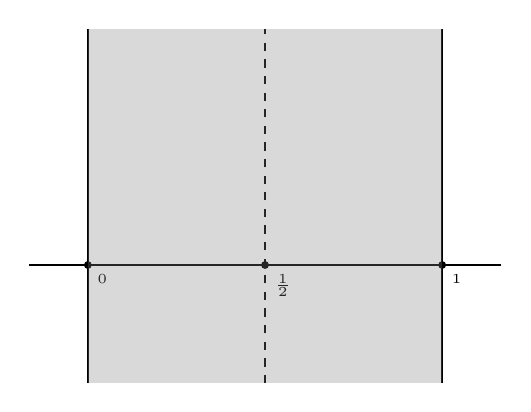
\begin{tikzpicture}[scale=1.5]
        \def\xmin{-0.5} \def\xmax{3.5}
        \def\ymin{-1} \def\ymax{2}
        \draw[thick] (\xmin,0) -- (\xmax,0);
        \draw[thick] (0,\ymin) -- (0,\ymax);
        \draw[thick] (3,\ymin) -- (3,\ymax);
        \draw[dashed] (1.5,\ymin) -- (1.5,\ymax);

        \node at (0,0) [below right] {\tiny{\(0\)}};
        \node at (0,0) [circle,fill,inner sep=1pt]{};
        \node at (1.5,0) [below right] {\tiny{\(\frac{1}{2}\)}};
        \node at (1.5,0) [circle,fill,inner sep=1pt]{};
        \node at (3,0) [below right] {\tiny{\(1\)}};
        \node at (3,0) [circle,fill,inner sep=1pt]{};

        \begin{scope}
          \path[clip] (0,\ymin) -- (0,\ymax) -- (3,\ymax) -- (3,\ymin) -- cycle;
          \fill[gray,opacity=0.3] (0,\ymin) rectangle (3,\ymax);
        \end{scope}
      \end{tikzpicture}
      \caption{The critical strip.}
      \label{fig:critical_strip}
    \end{figure}

    The \textbf{critical line}\index{critical line} is the vertical line left invariant by the transformation \(s \mapsto 1-s\) which is also given by \(\s = \frac{1}{2}\). The critical line bisects the critical strip vertically. The \textbf{central point}\index{central point} is the fixed point of the transformation \(s \mapsto 1-s\), in other words, the point \(s = \frac{1}{2}\). Clearly the central point is also the center of the critical line. The critical strip, critical line, and central point are all displayed in \cref{fig:critical_strip}.

    In the half-plane \(\s > 1\) we may study the analytic properties of \(L(s)\) via its Dirichlet series. Using the functional equation, we may write
    \[
      L(s) = \e_{L}q_{L}^{\frac{1}{2}-s}\frac{\g(1-s,L)}{\g(s,L)}\conj{L(1-\conj{s})}.
    \]
    This permits the study of \(L(s)\) in the half-plane \(\s < 0\) by using the Dirichlet series of \(\conj{L(1-\conj{s})}\) and the the functional equation data. The interior of the critical strip is exactly the region where we cannot use either of these methods to study the analytic properties of \(L(s)\). Of course, anything may be possible on the boundary lines \(\s = 0\) and \(\s = 1\) (for example Landau's theorem).
  \section{The Approximate Functional Equation}
    Despite not being able to study an analytic \(L\)-function \(L(s)\) in the critical strip by means of Dirichlet series, there is formula which acts as a compromise between the functional equation and the Dirichlet series. This formula is known as the approximate functional equation. The usefulness comes from the fact that the approximate functional equation is valid inside of the critical strip and therefore can be used to obtain analytic properties about \(L(s)\) in that region. We will first derive a preliminary result showing \(L(s)\) has at most polynomial growth.

    \begin{proposition}\label{prop:L_function_bounded_in_vertical_strips}
      Let \(L(s)\) be an analytic \(L\)-function with \(\s\) bounded and \(\s\) at least distance \(\e\) away from the possible pole at \(s = 1\). Then there is a positive constant \(A\) such that
      \[
        L(s) \ll_{\e} (|t|+3)^{A}.
      \]
    \end{proposition}
    \begin{proof}
      Observe that \((s-1)^{m_{L}}L(s) \ll_{\e} (|t|+3)^{m_{L}}\) on the vertical line \(\s = \max(1+\e,\s_{2})\). Now suppose \(\s = \min(-\e,\s_{1})\). On this vertical line, the functional equation and \cref{equ:gamma_factor_analytic_conductor_estimate} together show
      \[
        L(s) \ll_{\e} \mf{q}(s,L)^{\frac{1}{2}-\s}\conj{L(1-\conj{s})}.
      \]
      Hence there exists a positive constant \(A''\) with
      \[
        (s-1)^{m_{L}}L(s) \ll_{\e} (|t|+3)^{A''},
      \]
      on the vertical line \(\s = \min(-\e,\s_{1})\). As \((s-1)^{m_{L}}L(s)\) is entire and of order \(1\), we can apply the Phragm\'en-Lindel\"of convexity principle to \((s-1)^{m_{L}}L(s)\) the vertical strip \(\min(-\e,\s_{1}) \le \s \le \max(1+\e,\s_{2})\). Whence there is a positive constant \(A'\) such that
      \[
        (s-1)^{m_{L}}L(s) \ll_{\e} (|t|+3)^{A'},
      \]
      provided \(\s\) is bounded. Assuming \(s\) is at least distance \(\e\) away from the possible pole at \(s = 1\), diving by \((s-1)^{m_{L}}\) completes the proof.
    \end{proof}

    We are almost ready to prove the approximate function equation for an analytic \(L\)-function \(L(s)\). The formula itself consists of two sums representing the Dirichlet series at \(s\) and a dualized Dirichlet series at \(1-s\) as well as a potential residue term. The dual sum comes equip with a term containing the data of the functional equation. Both sums will also be dampened by a smooth cutoff function. In the statement of the approximate function equation, we will make use of a test function \(\Phi(u)\). We require \(\Phi(u)\) be an even holomorphic function bounded in the vertical strip \(|\tau| < a+1\) for some \(a > 1\) and such that \(\Phi(0) = 1\). For \(s\) in the critical strip, we let \(V_{s}(y,L)\) be the inverse Mellin transform
    \[
      V_{s}(y,L) = \frac{1}{2\pi i}\int_{(a)}\frac{\g(s+u,L)}{\g(s,L)}\Phi(u)y^{-u}\frac{du}{u},
    \]
    defined for \(y > 0\). Stirling's formula (see \cref{sec:the_gamma_function}) implies
    \[
      \frac{\G(s+u)}{\G(s)} \ll_{\e} \frac{(|t+r|+3)^{\s+\tau-\frac{1}{2}}}{(|t|+3)^{\s-\frac{1}{2}}}e^{-\frac{\pi}{2}(|t+r|-|t|)},
    \]
    for \(s\) in the critical strip and bounded \(\tau\) provided \(s+u\) is at least distance \(\e\) away from the poles of the gamma function. Whence
    \begin{equation}\label{equ:gamma_factor_s_and_u_estimate}
      \frac{\g(s+u,L)}{\g(s,L)} \ll_{\e} \frac{\mf{q}_{\infty}(s+u,L)^{\frac{\s+\tau}{2}-\frac{1}{4}}}{\mf{q}_{\infty}(s,L)^{\frac{\s}{2}-\frac{1}{4}}}e^{-d_{L}\frac{\pi}{2}(|t+r|-|t|)},
    \end{equation}
    for \(s\) in the critical strip and bounded \(\tau\) provided \(s+u\) is at least distance \(\e\) away from the poles of the gamma factor. Since \(\Phi(u)\) is bounded in the vertical strip \(|\tau| < a+1\), the integrand exhibits exponential decay. Therefore the integral is locally absolutely uniformly convergent and hence \(V_{s}(y,L)\) is smooth. The function \(V_{s}(y,L)\) is the smooth cutoff function mentioned previously. We will also let \(\e(s,L)\) be given by
    \[
      \e(s,L) = \e_{L}q_{L}^{\frac{1}{2}-s}\frac{\g(1-s,L)}{\g(s,L)}.
    \]
    This term appears as a factor in the dual sum accounting for the functional equation data. Lastly, we set
    \[
      R(s,X,L) = \Res_{u = 1-s}\frac{\L(s+u,L)\Phi(u)X^{u}}{u}+\Res_{u = -s}\frac{\L(s+u,L)\Phi(u)X^{u}}{u}.
    \]
    This is the potential residue term that appears in the approximate functional equation. Observe that it vanishes provided \(s \neq 0,1\). We now prove the \textbf{approximate function equation}\index{approximate function equation} for \(L(s)\).

    \begin{theorem*}[Approximate functional equation]
      Suppose \(L(s)\) is an analytic \(L\)-function, \(\Phi(u)\) is an even holomorphic function bounded in the vertical strip \(|\tau| < a+1\) for some \(a > 1\) and such that \(\Phi(0) = 1\), and let \(X > 0\). Then for \(s\) in the critical strip, we have
      \[
        L(s) = \sum_{n \ge 1}\frac{a_{L}(n)}{n^{s}}V_{s}\left(\frac{n}{\sqrt{q_{L}}X},L\right)+\e(s,L)\sum_{n \ge 1}\frac{\conj{a_{L}(n)}}{n^{1-s}}V_{1-s}\left(\frac{nX}{\sqrt{q_{L}}},L\right)+\frac{R(s,X,L)}{q_{L}^{\frac{s}{2}}\g(s,L)}.
      \]
    \end{theorem*}
    \begin{proof}
      Consider the integral
      \[
        \frac{1}{2\pi i}\int_{(a)}\L(s+u,L)\Phi(u)X^{u}\,\frac{du}{u}.
      \]    
      Stirling's formula (see \cref{sec:the_gamma_function}) shows that \(\g(s+u,L)\) exhibits exponential decay while \(L(s+u)\) has at most polynomial growth by \cref{prop:L_function_bounded_in_vertical_strips}. Since \(\Phi(u)\) is bounded in the vertical strip \(|\tau| < a+1\), it follows that the integrand exhibits exponential decay. Therefore the integral is locally absolutely uniformly convergent. We will evaluate the integral in two ways. On the one hand, we can expand \(L(s+u)\) inside the integrand as a Dirichlet series and by absolute boundedness of the integral we may interchange the sum and integral. A short computation shows that this is
      \[
        q_{L}^{\frac{s}{2}}\g(s,L)\sum_{n \ge 1}\frac{a_{L}(n)}{n^{s}}V_{s}\left(\frac{n}{\sqrt{q_{L}}X},L\right).
      \]
      On the other hand, we can shift the line of integration to \((-a)\). In doing so we pass by a simple pole at \(u = 0\) and possible poles at \(u = 1-s\) and \(u = -s\) giving
      \[
        \frac{1}{2\pi i}\int_{(-a)}\L(s+u,L)\Phi(u)X^{u}\,\frac{du}{u}+\L(s,L)+R(s,X,L).
      \]
      Apply the functional equation and perform the change of variables \(u \mapsto -u\) to rewrite this as
      \[
        -\e_{L}\frac{1}{2\pi i}\int_{(a)}\L(1-(s+u),\conj{L})\Phi(u)X^{-u}\,\frac{du}{u}+\L(s,L)+R(s,X,L).
      \]
      Analogous to the above, we can now expand \(\conj{L}(1-(s+u))\) inside the integrand as a Dirichlet series and by absolute boundedness of the integral we may interchange the sum and integral. A short computation shows that our previous expression becomes
      \[
        -\e_{L}q_{L}^{\frac{1-s}{2}}\g(1-s,L)\sum_{n \ge 1}\frac{\conj{a_{L}(n)}}{n^{1-s}}V_{s}\left(\frac{nX}{\sqrt{q_{L}}},L\right)+\L(s,L)+R(s,X,L).
      \]
      Equating these two evaluations and isolating the completion gives
      \begin{align*}
        \L(s,L) &= q_{L}^{\frac{s}{2}}\g(s,L)\sum_{n \ge 1}\frac{a_{L}(n)}{n^{s}}V_{s}\left(\frac{n}{\sqrt{q_{L}}X},L\right) \\
        &+ \e_{L}q_{L}^{\frac{1-s}{2}}\g(1-s,L)\sum_{n \ge 1}\frac{\conj{a_{L}(n)}}{n^{1-s}}V_{1-s}\left(\frac{nX}{\sqrt{q_{L}}},L\right)+R(s,X,L).
      \end{align*}
      Diving by \(q_{L}^{\frac{s}{2}}\g(s,L)\) completes the proof.
    \end{proof}

    Let us now show how \(V_{s}(y,L)\) has the effect of dampening the two dual sums appearing on the right-hand side of the approximate functional equation. In practice, it is common to choose \(\Phi(u)\) such that it has exponential decay and we can make the vertical strip on which it is bounded arbitrarily wide. For example, let
    \[
      \Phi(u) = \cos^{-4d_{L}M}\left(\frac{\pi u}{4M}\right),
    \]
    for some positive integer \(M\). Clearly \(\Phi(u)\) is an even holomorphic function in the vertical strip \(|\tau| < (2M-1)+1\) and satisfies \(\Phi(0) = 1\). In view of the identity \(\cos(u) = \frac{e^{iu}+e^{-iu}}{2}\), we find that
    \begin{equation}\label{equ:choice_for_V_decay_estimate}
     \cos^{-4d_{L}M}\left(\frac{\pi u}{4M}\right) \ll_{\e} e^{-d_{L}\pi|r|},
    \end{equation}
    for \(|\tau| < (2M-1)+1\) provided \(u\) is at least distance \(\e\) away from the poles of \(\Phi(u)\). Therefore \(\Phi(u)\) admits exponential decay. For this choice of \(\Phi(u)\), \(V_{s}(y,L)\) and its derivatives will possess rapid decay.

    \begin{proposition}\label{prop:V_function_decay}
      Let \(L(s)\) be an analytic \(L\)-function, set \(\Phi(u) = \cos^{-4d_{L}M}\left(\frac{\pi u}{4M}\right)\) for some positive integer \(M\), and let \(V_{s}(y,L)\) be the inverse Mellin transform defined by
      \[
        V_{s}(y,L) = \frac{1}{2\pi i}\int_{(2M-1)}\frac{\g(s+u,L)}{\g(s,L)}\Phi(u)y^{-u}\frac{du}{u}.
      \]
      Then for \(s\) in the critical strip, any nonnegative integer \(k\), and positive integer \(N\) with \(N < 2M\), \(V_{s}(y,L)\) satisfies the estimates
      \[
        (-y)^{k}V_{s}^{(k)}(y,L) = \begin{cases} \d_{k,0}+O_{\e}\left(\left(\frac{y}{\sqrt{\mf{q}_{\infty}(s,L)}}\right)^{N}\right) & \text{if \(y \ll \sqrt{\mf{q}_{\infty}(s,L)}\)}, \\ O_{\e}\left(\left(\frac{y}{\sqrt{\mf{q}_{\infty}(s,L)}}\right)^{-N}\right) & \text{if \(y \gg \sqrt{\mf{q}_{\infty}(s,L)}\)}. \end{cases}
      \]
      In particular,
      \[
        (-y)^{k}V_{s}^{(k)}(y,L) \ll_{\e} \left(1+\frac{y}{\sqrt{\mf{q}_{\infty}(s,L)}}\right)^{-N}.
      \]
    \end{proposition}
    \begin{proof}
      As we have already seen, the integrand defining \(V_{s}(y,L)\) admits exponential decay. This permits us to differentiate under the integral sign and shift the line of integration. The former shows
      \[
        (-y)^{k}V_{s}^{(k)}(y,L) = \frac{1}{2\pi i}\int_{(2M-1)}\frac{\g(s+u,L)}{\g(s,L)}\Phi(u)(u)_{k}y^{-u}\frac{du}{u}.
      \]
      Shifting to \((-N)\), we pass by a simple pole at \(u = 0\) of residue \(1\) if and only if \(k = 0\). This gives
      \[
        (-y)^{k}V_{s}^{(k)}(y,L) = \d_{k,0}+\frac{1}{2\pi i}\int_{(-N)}\frac{\g(s+u,L)}{\g(s,L)}\Phi(u)(u)_{k}y^{-u}\frac{du}{u}.
      \]
      This integrand also exhibits exponential decay since the Pochhammer symbol grows polynomially. Therefore the integral is dominated by the contribution when \(u \ll 1\) and the \cref{equ:gamma_factor_s_and_u_estimate,equ:choice_for_V_decay_estimate} together show
      \[
        (-y)^{k}V_{s}^{(k)}(y,L) = \d_{k,0}+O_{\e}\left(\left(\frac{y}{\sqrt{\mf{q}_{\infty}(s,L)}}\right)^{N}\right).
      \]
      If we instead shift to \((N)\), we do not pass by any poles and obtain
      \[
        (-y)^{k}V_{s}^{(k)}(y,L) = \frac{1}{2\pi i}\int_{(N)}\frac{\g(s+u,L)}{\g(s,L)}\Phi(u)(u)_{k}y^{-u}\frac{du}{u}.
      \]
      An analogous argument to estimate the remaining integral shows
      \[
        (-y)^{k}V_{s}^{(k)}(y,L) = O_{\e}\left(\left(\frac{y}{\sqrt{\mf{q}_{\infty}(s,L)}}\right)^{-N}\right).
      \]
      From these \(O\)-estimates we obtain nontrivial bounds in the ranges \(y \ll \sqrt{\mf{q}_{\infty}(s,L)}\) and \(y \gg \sqrt{\mf{q}_{\infty}(s,L)}\) respectively. Combining both of these estimates produces the bound
      \[
        (-y)^{k}V_{s}^{(k)}(y,L) \ll_{\e} \left(1+\frac{y}{\sqrt{\mf{q}_{\infty}(s,L)}}\right)^{-N}.
      \]
    \end{proof}

    With our choice of \(\Phi(u)\), this result shows that \(V_{s}(y,L)\) is essentially \(1\) for \(y \ll \sqrt{\mf{q}_{\infty}(s,L)}\) and has rapid decay thereafter as we can take \(M\) (and hence \(N\)) to be arbitrarily large.
    
    In a similar spirit to the approximate functional equation, a useful summation formula can be derived from the functional equation. Let \(\psi(y)\) be a smooth weight where \(\Psi(s)\) is its Mellin transform. Then we will let \(\psi(y,L)\) be the inverse Mellin transform
    \[
      \psi(y,L) = \frac{1}{2\pi i}\int_{(a)}q_{L}^{s}\frac{\g(s,L)}{\g(1-s,L)}y^{-s}\Psi(1-s)\,ds,
    \]
    defined for \(y > 0\) where \(a > 1\). By our choice of \(\psi(y)\), its inverse Mellin transform \(\Psi(s)\) has rapid decay. Since \(L(s)\) has at most polynomial growth by \cref{prop:L_function_bounded_in_vertical_strips}, the integrand has rapid decay as well. Therefore the integral is locally absolutely uniformly convergent and hence \(\psi(y,L)\) is smooth for \(y > 0\). We will also set
    \[
      R_{L} = \Res_{s = 1}L(s).
    \]
    Our result is the following:

    \begin{theorem}
      Let \(L(s)\) be an analytic \(L\)-function and let \(\psi(y)\) be a smooth weight where \(\Psi(s)\) is its Mellin transform. Then
      \[
        \sum_{n \ge 1}a_{L}(n)\psi(n) = \frac{\e_{L}}{\sqrt{q_{L}}}\sum_{n \ge 1}\conj{a_{L}(n)}\psi(n,L)+R_{L}\Psi(1).
      \]
    \end{theorem}
    \begin{proof}
      Smoothed Perron's formula implies
      \[
        \sum_{n \ge 1}a_{L}(n)\psi(n) = \frac{1}{2\pi i}\int_{(a)}L(s)\Psi(s)\,ds.
      \]
      By our choice of \(\psi(y)\), its inverse Mellin transform \(\Psi(s)\) has rapid decay. Since \(L(s)\) has at most polynomial growth by \cref{prop:L_function_bounded_in_vertical_strips}, the integrand has rapid decay as well. Therefore the integral is locally absolutely uniformly convergent which permits us to shift the line of integration. Shifting to \((1-a)\), we pass by a potential pole at \(s = 1\) and obtain
      \[
        \sum_{n \ge 1}a_{L}(n)\psi(n) = \frac{1}{2\pi i}\int_{(1-a)}L(s)\Psi(s)\,ds+R_{L}\Psi(1).
      \]
      Apply the functional equation to rewrite this equality in the form
      \[
        \sum_{n \ge 1}a_{L}(n)\psi(n) = \frac{1}{2\pi i}\int_{(1-a)}\e_{L}q_{L}^{\frac{1}{2}-s}\frac{\g(1-s,L)}{\g(s,L)}\conj{L(1-\conj{s})}\Psi(s)\,ds+R_{L}\Psi(1).
      \]
      Performing the change of variables \(s \mapsto 1-s\) in this latter integral gives
      \[
        \sum_{n \ge 1}a_{L}(n)\psi(n) = \frac{1}{2\pi i}\int_{(a)}\e_{L}q_{L}^{s-\frac{1}{2}}\frac{\g(s,L)}{\g(1-s,L)}\conj{L(\conj{s})}\Psi(1-s)\,ds+R_{L}\Psi(1).
      \]
      The proof is complete upon expanding \(\conj{L(\conj{s})}\) as a Dirichlet series, interchanging the sum and integral by absolute boundedness of the integral, and factoring out \(\frac{\e_{L}}{\sqrt{q_{L}}}\).
    \end{proof}
  \section{The Riemann Hypothesis and Nontrivial Zeros}
    The zeros of an analytic \(L\)-functions \(L(s)\) has interesting behavior. From the Euler product we immediately see that \(L(s)\) has no zeros in the half-plane \(\s > 1\). We can use the functional equation to determine the zeros for \(\s < 0\). Indeed, write the functional equation in the form
    \[
      L(s) = \e_{L}q_{L}^{\frac{1}{2}-s}\frac{\g(1-s,L)}{\g(s,L)}\conj{L(1-\conj{s})}.
    \] 
    So for \(\s < 0\), we see that \(\conj{L(1-\conj{s})}\) is nonzero. Moreover, \(\g(1-s,L)\) is as well. Together this means that for \(\s < 0\) the poles of \(\g(s,L)\) are zeros of \(L(s)\). Such a zero is called a \textbf{trivial zero}\index{trivial zero} of \(L(s)\). From the definition of the gamma factor, they are all simple and of the form \(s = -(\mu_{j}+2n)\) for some gamma parameter \(\mu_{j}\) and nonnegative integer \(n\).
    
    Any other zero of \(L(s)\) is called a \textbf{nontrivial zero}\index{nontrivial zero} and it necessarily lies inside of the critical strip. Let \(\rho\) be a nontrivial zero of \(L(s)\). Then the functional equation implies that \(1-\conj{\rho}\) is also a nontrivial zero of \(L(s)\). This means that nontrivial zeros occur in pairs
    \[
      \rho \quad \text{and} \quad 1-\conj{\rho}.
    \]

    \begin{figure}[ht]
      \centering
      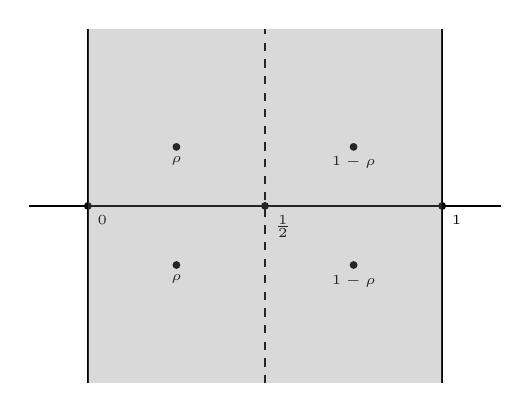
\begin{tikzpicture}[scale=1.5]
        \def\xmin{-0.5} \def\xmax{3.5}
        \def\ymin{-1.5} \def\ymax{1.5}
        \draw[thick] (\xmin,0) -- (\xmax,0);
        \draw[thick] (0,\ymin) -- (0,\ymax);
        \draw[thick] (3,\ymin) -- (3,\ymax);
        \draw[dashed] (1.5,\ymin) -- (1.5,\ymax);

        \node at (2.25,0.5) [circle,fill,inner sep=1pt]{};
        \node at (2.25,0.5) [below] {\tiny{\(1-\conj{\rho}\)}};
        \node at (0.75,0.5) [circle,fill,inner sep=1pt]{};
        \node at (0.75,0.5) [below] {\tiny{\(\rho\)}};
        \node at (2.25,-0.5) [circle,fill,inner sep=1pt]{};
        \node at (2.25,-0.5) [below] {\tiny{\(1-\rho\)}};
        \node at (0.75,-0.5) [circle,fill,inner sep=1pt]{};
        \node at (0.75,-0.5) [below] {\tiny{\(\conj{\rho}\)}};

        \node at (0,0) [below right] {\tiny{\(0\)}};
        \node at (0,0) [circle,fill,inner sep=1pt]{};
        \node at (1.5,0) [below right] {\tiny{\(\frac{1}{2}\)}};
        \node at (1.5,0) [circle,fill,inner sep=1pt]{};
        \node at (3,0) [below right] {\tiny{\(1\)}};
        \node at (3,0) [circle,fill,inner sep=1pt]{};

        \begin{scope}
          \path[clip] (0,\ymin) -- (0,\ymax) -- (3,\ymax) -- (3,\ymin) -- cycle;
          \fill[gray,opacity=0.3] (0,\ymin) rectangle (3,\ymax);
        \end{scope}
        \end{tikzpicture}
      \caption{Symmetric nontrivial zeros.}
      \label{fig:symmetric_nontrivial_zeros}
    \end{figure}

    It is possible to say more when \(L(s)\) takes real values for \(s > 1\). For in this case, the Schwarz reflection principle implies \(L(\conj{s}) = \conj{L(s)}\) and that \(L(s)\) takes real values on the entire real line save for the possible pole at \(s = 1\). It follows from the functional equation that \(\conj{\rho}\) and \(1-\rho\) are also nontrivial zeros. Therefore the nontrivial zeros of \(L(s)\) come in sets of four
    \[
      \rho, \quad \conj{\rho}, \quad 1-\rho, \quad \text{and} \quad 1-\conj{\rho},
    \]
    as displayed in \cref{fig:symmetric_nontrivial_zeros}.

    The \textbf{Riemann hypothesis}\index{Riemann hypothesis} for \(L(s)\) says that this symmetry should be as simple as possible.

    \begin{conjecture*}[Riemann hypothesis]
      All of the nontrivial zeros of the analytic \(L\)-function \(L(s)\) lie on the vertical line \(\s = \frac{1}{2}\).
    \end{conjecture*}

    While stated as a conjecture, we not expect the Riemann hypothesis to hold for just any analytic \(L\)-function. We do however expect it to hold for Selberg class \(L\)-functions. In particular, the \textbf{Selberg class Riemann hypothesis}\index{Selberg class Riemann hypothesis} says that this symmetry should hold for any Selberg class \(L\)-function:

    \begin{conjecture*}[Selberg class Riemann hypothesis]
      All of nontrivial zeros of any Selberg class \(L\)-function \(L(s)\) lie on the vertical line \(\s = \frac{1}{2}\).
    \end{conjecture*}

    So far, the Riemann hypothesis remains completely out of reach for any analytic \(L\)-function and thus the Selberg class Riemann hypothesis does as well.
  \section{The Lindel\"of Hypothesis and Estimates on the Critical Line}
    Instead of asking about the zeros of an analytic \(L\)-function \(L(s)\) on the critical line we can ask about its growth there. Let us begin this investigation by deriving an upper bound for \(L(s)\) on the critical line using the Phragm\'en-Lindel\"of convexity principle. This amounts to a more refined version of the argument used in \cref{prop:L_function_bounded_in_vertical_strips} for the critical strip.

    \begin{theorem}\label{thm:convexity_bound_for_L_function_in_critial_strip}
      Let \(L(s)\) be an analytic \(L\)-function. Then for \(-\e \le \s \le 1+\e\), we have
      \[
        L(s) \ll_{\e} \mf{q}(s,L)^{\frac{1-\s}{2}+\e},
      \]
      provided \(s\) is at least distance \(\e\) away from the possible pole at \(s = 1\).
    \end{theorem}
    \begin{proof}
      Since \((s-1)^{m_{L}}L(s)\) is entire and of order \(1\), we will apply the Phragm\'en-Lindel\"of convexity principle just outside the edges of the critical strip. Just past the right edge along the vertical line \(\s = 1+\e\), we have
      \[
        (s-1)^{m_{L}}L(s) \ll_{\e} (s-1)^{m_{L}}.
      \]
      Just past the left edge along the vertical line \(\s = -\e\), the functional equation and \cref{equ:gamma_factor_analytic_conductor_estimate} together imply the bound
      \[
        (s-1)^{m_{L}}L(s) \ll_{\e} (s-1)^{m_{L}}\mf{q}(s,L)^{\frac{1}{2}+\e}.
      \]
      By the Phragm\'en-Lindel\"of convexity principle, we obtain
      \[
        (s-1)^{m_{L}}L(s) \ll_{\e} (s-1)^{m_{L}}\mf{q}(s,L)^{\frac{1-\s}{2}+\e},
      \]
      provided \(-\e \le \s \le 1+\e\). Assuming \(s\) is at least distance \(\e\) away from the possible pole at \(s = 1\), dividing by \((s-1)^{m_{L}}\) completes the proof.
    \end{proof}
    
    At the critical line this theorem produces the bound
    \[
      L\left(\frac{1}{2}+it\right) \ll_{\e} \mf{q}\left(\frac{1}{2}+it,L\right)^{\frac{1}{4}+\e}.
    \]
    This is known as the \textbf{convexity bound}\index{convexity bound} for \(L(s)\). The \textbf{Lindel\"of hypothesis}\index{Lindel\"of hypothesis} for \(L(s)\) says that the exponent can be reduced to \(\e\):

    \begin{conjecture*}[Lindel\"of hypothesis]
      The analytic \(L\)-function \(L(s)\) satisfies
      \[
        L\left(\frac{1}{2}+it\right) \ll_{\e} \mf{q}\left(\frac{1}{2}+it,L\right)^{\e}.
      \]
    \end{conjecture*}

    Unlike the Riemann hypothesis, the Lindel\"of hypothesis is expected to hold for any analytic \(L\)-function. In any case, the \textbf{Selberg class Lindel\"of hypothesis}\index{Selberg class Lindel\"of hypothesis} says that the exponent can be reduced to \(\e\) for any Selberg class \(L\)-function:

    \begin{conjecture*}[Selberg class Lindel\"of hypothesis]
      Any Selberg class \(L\)-function \(L(s)\) satisfies
      \[
        L\left(\frac{1}{2}+it\right) \ll_{\e} \mf{q}\left(\frac{1}{2}+it,L\right)^{\e}.
      \]
    \end{conjecture*}

    Like the Riemann hypothesis, we have been unable to prove the Lindel\"of hypothesis for any analytic \(L\)-function. However, in practice the Lindel\"of hypothesis is more tractable. Generally speaking, any improvement upon the exponent in the convexity bound in any aspect of the analytic conductor is called a \textbf{subconvexity estimate}\index{subconvexity estimate} (or a \textbf{convexity breaking bound}\index{convexity breaking bound}). In the uniform case, we would like to prove bounds of the form
    \[
      L\left(\frac{1}{2}+it\right) \ll_{\e} \mf{q}\left(\frac{1}{2}+it,L\right)^{\d+\e},
    \]
    for some \(0 \le \d \le \frac{1}{4}\). The convexity bound says that we may take \(\d = \frac{1}{4}\) while the Lindel\"of hypothesis for \(L(s)\) implies that we may take \(\d = 0\). Any uniform subconvexity estimate would give a \(\d\) strictly less than \(\frac{1}{4}\). Subconvexity estimates are viewed with great interest. This is primarily because of their connection to the Lindel\"of hypothesis, but also because any improvement upon the convexity bound in any aspect of the analytic conductor often has drastic consequences in applications.

    \begin{remark}
      Some subconvexity bounds are deserving of names. The cases \(\d = \frac{3}{16}\) and \(\d = \frac{1}{6}\) are referred to as the \textbf{Burgess bound}\index{Burgess bound} and \textbf{Weyl bound}\index{Weyl bound} respectively.
    \end{remark}
    
    With a little more work, we can obtain a a similar bound for the derivatives of analytic \(L\)-functions. First observe that \cref{thm:convexity_bound_for_L_function_in_critial_strip} gives the estimate
    \[
      L(s) \ll_{\e} \mf{q}\left(\frac{1}{2}+it,L\right)^{\frac{1}{4}+\e},
    \]
    in the vertical strip \(\left|\s-\frac{1}{2}\right| \le \frac{\e}{2}\). This is just slightly stronger than the convexity bound. By Cauchy's integral formula, we may write
    \[
      L^{(k)}\left(\frac{1}{2}+it\right) = \frac{k!}{2\pi i}\int_{\eta}\frac{L(s)}{(s-\frac{1}{2}-it)^{k+1}}\,ds,
    \]
    where \(\eta\) is the circle about \(\frac{1}{2}+it\) of radius \(\frac{\e}{2}\). The parameterization \(u \mapsto \frac{1}{2}+it+\frac{\e}{2}e^{i\t}\) for \(\eta\) shows that
    \[
      L^{(k)}\left(\frac{1}{2}+it\right) \ll_{\e} \mf{q}\left(\frac{1}{2}+it,L\right)^{\frac{1}{4}+\e}.
    \]
    This is known as the \textbf{convexity bound}\index{convexity bound} for \(L^{(k)}(s)\).

    We now turn to the question of how to obtain estimates on the critical line. There are many methods one can apply often depending upon the particular analytic \(L\)-function of interest. Here we will provide a method that works in vast generality and reduces the estimation of \(L\left(\frac{1}{2}+it\right)\) to that of estimating smoothed finite sums of coefficients. To achieve this we need to establish the existence of certain bump functions. We say that a function \(\w(y)\) is a \textbf{smooth dyadic weight}\index{smooth dyadic weight} if it is a positive bump function supported in \([1-\d,2+\d]\) and such that
    \[
      \sum_{k \in \Z}\w\left(\frac{y}{2^{k}}\right) = 1,
    \]
    for positive \(y\). This last condition means \(\left(\w\left(\frac{y}{2^{k}}\right)\right)_{k \in \Z}\) is a partition of unity on \((0,\infty)\). To see that dyadic weights exist, let \(\psi(y)\) be a smooth weight that is identically \(1\) on \([1,2]\) and supported in \([1-\d,2+\d]\). Write
    \[
      \s(y) = \sum_{k \in \Z}\psi\left(\frac{y}{2^{k}}\right).
    \]
    Then \(\s(y)\) is finite as finitely many of its summands are nonzero since any positive \(y\) satisfies \(2^{k} \le y < 2^{k+1}\) for some unique integer \(k\). This forces \(\s(y)\) to be smooth and bounded. It is also bounded away from zero as \(\s(y) \ge 1\) because \(\psi(y)\) is identically \(1\) on \([1,2]\). Then we may take
    \[
      \w(y) = \frac{\psi(y)}{\s(y)}.
    \]
    This shows that smooth dyadic weights exist. For any \(t \in \R\) and \(X > 0\), set
    \[
      A_{\w}(t,X,L) = \sum_{n \ge 1}a_{L}(n)n^{-it}\w\left(\frac{n}{X}\right).
    \]
    For convenience, we will also let
    \[
      A_{\w}(X,L) = A_{\w}(0,X,L).
    \]
    Our result estimates \(L(s)\) at \(s = \frac{1}{2}+it\) in terms of \(A_{\w}(t,X,L)\).

    \begin{theorem}\label{thm:critical_line_estimate}
      Let \(L(s)\) be an analytic \(L\)-function and let \(\w(y)\) be a smooth dyadic weight. Then
      \[
        L\left(\frac{1}{2}+it\right) \ll_{\e} \mf{q}\left(\frac{1}{2}+it,L\right)^{\e}\sup_{X \ll \sqrt{\mf{q}\left(\frac{1}{2}+it,L\right)}}\left(\frac{|A_{\w}(t,X,L)|}{\sqrt{X}}\right).
      \]
    \end{theorem}
    \begin{proof}
      Take \(s = \frac{1}{2}+it\), \(X = 1\), and \(\Phi(u) = \cos^{-4d_{L}M}\left(\frac{\pi u}{4M}\right)\) for some large positive integer \(M\) in the approximate functional equation. This permits us to write
      \begin{align*}
        L\left(\frac{1}{2}+it\right) &= \sum_{n \ge 1}\frac{a_{L}(n)n^{-it}}{\sqrt{n}}V_{\frac{1}{2}+it}\left(\frac{n}{\sqrt{q_{L}}},L\right) \\
        &+ \e\left(\frac{1}{2}+it,L\right)\sum_{n \ge 1}\frac{\conj{a_{L}(n)}n^{it}}{\sqrt{n}}V_{\frac{1}{2}+it}\left(\frac{n}{\sqrt{q_{L}}},L\right)+\frac{R\left(\frac{1}{2}+it,1,L\right)}{q_{L}^{\frac{1}{4}+i\frac{t}{2}}\g\left(\frac{1}{2}+it,L\right)}.
      \end{align*}
      \cref{equ:gamma_factor_analytic_conductor_estimate} implies \(\e\left(\frac{1}{2}+it,L\right) \ll 1\) while \cref{equ:vertical_strip_gamma_estimates,equ:choice_for_V_decay_estimate} together imply that the residue term exhibits exponential decay. This implies that right-hand side of the approximate functional equation is
      \begin{align*}
        O\left(\sum_{n \ge 1}\frac{a_{L}(n)n^{-it}}{\sqrt{n}}V_{\frac{1}{2}+it}\left(\frac{n}{\sqrt{q_{L}}},L\right)\right)+O\left(\sum_{n \ge 1}\frac{\conj{a_{L}(n)}n^{it}}{\sqrt{n}}V_{\frac{1}{2}-it}\left(\frac{n}{\sqrt{q_{L}}},L\right)\right)+O(e^{-|t|}).
      \end{align*}
      We now turn to estimating the remaining sums which will be accomplished by applying the smooth dyadic weight. Consider the first sum. By our choice of \(\Phi(u)\), the estimates in \cref{prop:V_function_decay} are valid which implies that the summands exhibit rapid decay for \(n \gg \sqrt{\mf{q}\left(\frac{1}{2}+it,L\right)}\). Whence the sum is say
      \[
        \sum_{n \ll \sqrt{\mf{q}\left(\frac{1}{2}+it,L\right)}}\frac{a_{L}(n)n^{-it}}{\sqrt{n}}V_{\frac{1}{2}+it}\left(\frac{n}{\sqrt{q_{L}}},L\right)+O_{\e}\left(\mf{q}\left(\frac{1}{2}+it,L\right)^{\e}\right)
      \]
      Now write 
      \[
        V_{s}(y,L) = \sum_{k \in \Z}\w\left(\frac{y}{2^{k}}\right)V_{s}(y,L).
      \]
      Apply this identity to the sum and interchange the resulting two sums by local finiteness to obtain
      \[
        \sum_{k \in \Z}\sum_{n \ll \sqrt{\mf{q}\left(\frac{1}{2}+it,L\right)}}\frac{a_{L}(n)n^{-it}}{\sqrt{n}}\w\left(\frac{n}{2^{k}\sqrt{q_{L}}}\right)V_{\frac{1}{2}+it}\left(\frac{n}{\sqrt{q_{L}}},L\right).
      \]
      By compact support of the smooth dyadic weight, for each \(k\) the inner sum over \(n\) is supported on the dyadic block \(n \asymp X_{k}\) where \(X_{k} = 2^{k}\sqrt{q_{L}}\). As \(n \ll \sqrt{\mf{q}\left(\frac{1}{2}+it,L\right)}\), the summands which contribute must satisfy \(k \ll \log\mf{q}_{\infty}\left(\frac{1}{2}+it,L\right)\). Therefore our double sum can be expressed as
      \[
        \sum_{k \ll \log\mf{q}_{\infty}\left(\frac{1}{2}+it,L\right)}\sum_{n \asymp X_{k}}\frac{a_{L}(n)n^{-it}}{\sqrt{n}}\w\left(\frac{n}{X_{k}}\right)V_{\frac{1}{2}+it}\left(\frac{n}{\sqrt{q_{L}}},L\right).
      \]
      Let \(V(y) = \frac{1}{\sqrt{y}}V_{\frac{1}{2}+it}\left(\frac{y}{\sqrt{q_{L}}},L\right)\). By Abel summation, the inner sum is \(O\) of
      \[
        \sup_{n \asymp X_{k}}|A_{\w}(X_{k},t,L)|\left|V(n)\right|+\int_{u \asymp X_{k}}|A_{\w}(u,t,L)||V'(u)|\,du.
      \]
      In view of \cref{prop:V_function_decay}, we have the estimates
      \[
        V(y) = O\left(\frac{1}{\sqrt{y}}\right) \quad \text{and} \quad V'(y) = O\left(\frac{1}{y^{\frac{3}{2}}}\right),
      \]
      for \(y \ll \sqrt{\mf{q}\left(\frac{1}{2}+it,L\right)}\). Whence our previous expression is \(O\) of
      \[
        \sup_{X \asymp X_{k}}\left(\frac{|A_{\w}(t,X,L)|}{\sqrt{X}}\right).
      \]
      As there are \(O_{\e}\left(\mf{q}\left(\frac{1}{2}+it,L\right)^{\e}\right)\) many such \(k\), the bound above implies that our sum is \(O_{\e}\) of
      \[
        \mf{q}\left(\frac{1}{2}+it,L\right)^{\e}\sup_{X \ll \sqrt{\mf{q}\left(\frac{1}{2}+it,L\right)}}\left(\frac{|A_{\w}(t,X,L)|}{\sqrt{X}}\right).
      \]
      The estimate for the second sum is treated analogously. Thus
      \[
        L\left(\frac{1}{2}+it\right) \ll_{\e} \mf{q}\left(\frac{1}{2}+it,L\right)^{\e}\sup_{X \ll \sqrt{\mf{q}\left(\frac{1}{2}+it,L\right)}}\left(\frac{|A_{\w}(t,X,L)|}{\sqrt{X}}\right),
      \]
      upon absorbing smaller order \(O\)-estimates.
    \end{proof}

    As any useful estimate for the sum \(A_{\w}(t,X,L)\) will be in terms of powers of \(X\), the supremum in \cref{thm:central_value_estimate} will automatically pick out the largest possible bound when \(X\) is the square root of the analytic conductor. This means that the savings of \(\sqrt{X}\) in the denominator is essentially as large as possible. For example, we obtain the convexity bound as an application. Since the Dirichlet series of \(L(s)\) is absolutely convergent for \(\s < 1\), we have a bound of shape
    \[
      \sum_{n \le X}|a_{L}(n)| \ll_{\e} X^{1+\e}.
    \]
    Then \(A_{\w}(t,X,L) \ll_{\e} X^{1+\e}\) as well and we obtain
    \begin{equation}\label{equ:coefficient_sum_trivial_bound}
      \sup_{X \ll \sqrt{\mf{q}\left(\frac{1}{2}+it,L\right)}}\frac{|A_{\w}(t,X,L)|}{\sqrt{X}} \ll_{\e} \mf{q}\left(\frac{1}{2}+it,L\right)^{\frac{1}{4}+\e},
    \end{equation}
    which gives the convexity bound. As we believe \(L(s)\) satisfies the Lindel\"of hypothesis, we should expect lots of cancellation in the sum \(A_{\w}(t,X,L)\). In fact, the expected cancellation should be \(O\left(\mf{q}\left(\frac{1}{2}+it,L\right)^{\frac{1}{4}}\right)\) in light of the aforementioned bound. This means we expect \(A_{\w}(t,X,L)\) to exhibit square-root cancellation in the sense
    \[
      A_{\w}(t,X,L) \ll_{\e} X^{\frac{1}{2}+\e}.
    \]
    As the coefficients \(a_{L}(n)\) may very well be real, the expected cancellation must come from the terms \(n^{-it} = e^{-it\log(n)}\) which acts on the coefficients \(a_{L}(n)\) by rotation. In effect, we should think of the terms \(a_{L}(n)n^{-it}\) as modeling identically distributed random variables. 

    The case when \(t = 0\) deserves special interest as we are estimating the value of an analytic \(L\)-function at the central point. The value of \(L(s)\) at the central point is called the \textbf{central value}\index{central value} of \(L(s)\). Many important properties about an analytic \(L\)-function can be connected to its central value. Any argument used to estimate the central value of an analytic \(L\)-function is called a \textbf{central value estimate}\index{central value estimate}. Taking \(t = 0\) in \cref{thm:critical_line_estimate} gives a way to obtain central value estimates.

    \begin{theorem}\label{thm:central_value_estimate}
      Let \(L(s)\) be an analytic \(L\)-function and let \(\w(y)\) be a smooth dyadic weight. Then
      \[
        L\left(\frac{1}{2}\right) \ll_{\e} \mf{q}\left(\frac{1}{2},L\right)^{\e}\max_{X \ll \sqrt{\mf{q}\left(\frac{1}{2},L\right)}}\left(\frac{|A_{\w}(X,L)|}{\sqrt{X}}\right).
      \]
    \end{theorem}
    \begin{proof}
      Take \(t = 0\) in \cref{thm:critical_line_estimate}.
    \end{proof}
  \section{Moments}
    While both the Riemann and Lindel\"of hypotheses remain out of reach for any analytic \(L\)-function \(L(s)\), the latter is more tractable because the convexity bound gives the estimate
    \[
      L\left(\frac{1}{2}+it\right) \ll_{\e} \mf{q}\left(\frac{1}{2}+it,L\right)^{\d+\e},
    \]
    with \(\d = \frac{1}{4}\) whereas the Lindel\"of hypothesis claims that we can take \(\d = 0\). As we have already mentioned, breaking the convexity bound \(\d = \frac{1}{4}\) is a very daunting task requiring extremely modern techniques. This approach of breaking convexity to study the Lindel\"of hypothesis is quite direct. There is an indirect approach by considering averages of the analytic \(L\)-function in question. This is the study of moments of \(L\)-functions. For any analytic \(L\)-function \(L(s)\) and positive integer \(k\), we define the \(k\)-th \textbf{moment}\index{moment} of \(L(s)\), namely \(M_{k}(T,L)\), by
    \[
      M_{k}(T,L) = \int_{0}^{T}\left|L\left(\frac{1}{2}+it\right)\right|^{k}\,dt,
    \]
    for any positive \(T\). It is useful to think of \(M_{k}(T,L)\) as a \(k\)-th power average of \(L\left(\frac{1}{2}+it\right)\). One of the fundamental reasons why the study of moments is useful is that sufficient estimates for \(M_{2k}(T,L)\) in \(T\) is equivalent to the Lindel\"of hypothesis.

    \begin{proposition}\label{prop:equivalence_Lindelof_hypothesis_and_moments}
      Let \(L(s)\) be an analytic \(L\)-function. The truth of the Lindel\"of hypothesis for \(L(s)\) is equivalent to the estimate
      \[
        M_{2k}(T,L) \ll_{\e} T^{1+\e},
      \]
      for all positive integers \(k\).
    \end{proposition}
    \begin{proof}
      First suppose the Lindel\"of hypothesis for \(L(s)\) holds. Then we obtain the estimate
      \[
        M_{2k}(T,L) \ll_{\e} T^{1+\e},
      \]
      at once for all \(k\). Now suppose that \(M_{2k}(T,L) \ll_{\e} T^{1+\e}\) for all \(k\). If the Lindel\"of hypothesis for \(L(s)\) is false then there is some \(\d > 0\) and positive unbounded sequence \((t_{n})_{n \ge 1}\) such that
      \[
        \left|L\left(\frac{1}{2}+it_{n}\right)\right| > C\mf{q}\left(\frac{1}{2}+it_{n},L\right)^{\d},
      \]
      for any positive constant \(C\). In particular, we may write
        \[
        \left|L\left(\frac{1}{2}+it_{n}\right)\right| > Ct_{n}^{d_{L}\d}.
      \]
      The convexity bound for \(L(s)\) implies the weaker estimate \(\left|L'\left(\frac{1}{2}+it\right)\right| \le C't^{d_{L}}\) for some positive constant \(C'\) provided \(t\) is bounded away from zero. Now write
      \[
        \left|L\left(\frac{1}{2}+it\right)-L\left(\frac{1}{2}+it_{n}\right)\right| = \left|\int_{t_{n}}^{t}L'\left(\frac{1}{2}+ir\right)\,dr\right|.
      \]
      Taking \(C = 2C'\), a short computation using these results shows that
      \[
        \left|L\left(\frac{1}{2}+it\right)-L\left(\frac{1}{2}+it_{n}\right)\right| \le \frac{C}{2}t^{d_{L}\d},
      \]
      provided \(t\) is bounded away from zero and satisfies \(|t-t_{n}| \le t_{n}^{d_{L}(\d-1)}\). For such \(t\), it follows that
      \[
        \left|L\left(\frac{1}{2}+it\right)\right| > \frac{C}{2}t_{n}^{d_{L}\d}.
      \]
      Now take \(T = \frac{4}{3}t_{n}\) so that the interval \((t_{n}-t_{n}^{d_{L}(\d-1)},t_{n}+t_{n}^{d_{L}(\d-1)})\) is contained in \(\left(\frac{T}{2},T\right)\). Then
      \[
        M_{2k}(T,L) > 2\left(\frac{C}{2}\right)^{2k}\left(\frac{3}{4}\right)^{(2k+1)d_{L}\d-d_{L}}T^{(2k+1)d_{L}\d-d_{L}}.
      \]
      This is a contradiction for sufficiently large \(k\) which completes the proof.
    \end{proof}

    The usefulness of this result is that the difficulty of proving the Lindel\"of hypothesis for \(L(s)\) has been transferred to proving sufficient asymptotics for the moments \(M_{2k}(T,L)\) each of which should, heuristically speaking, be an easier problem to resolve on its own.
  \section{Logarithmic Derivatives}
    Recall that \(L(s)\) nonzero in the half-plane \(\s > 1\). As this region is simply connected, there exists a unique holomorphic logarithm \(\log L(s)\) there. By absolute convergence of the Euler product, we may write
    \[
      \log L(s) = -\sum_{p}\sum_{j}\log(1-\a_{j}(p)p^{-s}).
    \]
    Moreover, the bound \(|\a_{j}(p)| \le p^{\t_{L}}\) ensures that \(|\a_{j}(p)p^{-s}| < 1\) in this half-plane. Therefore the Taylor series of the logarithm is valid in this region and we may further write
    \[
      \log L(s) = \sum_{p}\sum_{j}\sum_{k \ge 1}\frac{\a_{j}(p)^{k}}{kp^{ks}}.
    \]
    While this triple sum converges for \(\s > 1\), the bound \(|\a_{j}(p)p^{-s}| < p^{\t_{L}-\s}\) only guarantees absolutely convergence for \(\s > 1+\t_{L}\). It is in this half-plane that we may differentiate termwise. A short computation shows
    \[
       \frac{L'}{L}(s) = -\sum_{n \ge 1}\frac{\L_{L}(n)}{n^{s}},
    \]
    where
    \[
      \L_{L}(n) = \begin{cases} \sum_{j}\a_{j}(p)^{k}\log(p) & \text{if \(n = p^{k}\)}, \\ 0 & \text{otherwise}. \end{cases}
    \]
    We call \(\L_{L}(n)\) the \textbf{von Mangoldt coefficients}\index{von Mangoldt coefficients} of \(L(s)\). Also observe that the dual satisfies \(\L_{\conj{L}}(n) = \conj{\L_{L}(n)}\).

    There is an incredibly useful formula for the logarithmic derivative of \(L(s)\) which is often the starting point for deeper analytic investigations. To deduce it, we require a more complete understanding of the completion \(\L(s,L)\). First observe that the zeros \(\rho\) of \(\L(s,L)\) are contained within the critical strip. Indeed, by our earlier discussion of zeros, \(\L(s,L)\) is nonzero for \(\s > 1\) and the functional equation implies that \(\L(s,L)\) is nonzero for \(\s < 0\) too. This means that the zeros of \(\L(s,L)\) are exactly nontrivial zeros of \(L(s)\). Now let us setup some notation. We define \(\xi(s,L)\) by
    \[
      \xi(s,L) = (s(1-s))^{m_{L}}\L(s,L).
    \]
    Observe that the dual satisfies \(\xi(s,\conj{L}) = \conj{\xi(\conj{s},L)}\). In any case, the functional equation implies
    \begin{equation}
      \xi(s,L) = \e_{L}\conj{\xi(1-\conj{s},L)},
    \end{equation}
    which we refer to as the \textbf{functional equation}\index{functional equation} for \(\xi(s,L)\). Now \(\xi(s,L)\) is just \(\L(s,L)\) with the potential poles at \(s = 0\) and \(s = 1\) removed. This means \(\xi(s,L)\) is entire. In fact, it admits a Hadamard factorization. To see this, first observe that \(\xi(s,L)\) is of order \(1\) by Stirling's formula (see \cref{sec:the_gamma_function}) and that \((s-1)^{m_{L}}L(s)\) is of order \(1\). Then the Hadamard factorization theorem implies
    \[
      \xi(s,L) = e^{A_{L}+B_{L}s}\prod_{\rho \neq 0,1}\left(1-\frac{s}{\rho}\right)e^{\frac{s}{\rho}},
    \]
    for some constants \(A_{L}\) and \(B_{L}\) and that the sum
    \begin{equation}\label{Hadamard_zero_sum_for_xi}
      \sum_{\rho \neq 0,1}\frac{1}{|\rho|^{1+\e}},
    \end{equation}
    is convergent. Our next result will utilize the Hadamard factorization of \(\xi(s,L)\) to produce a formula relating the logarithmic derivative of \(L(s)\) to its zeros.

    \begin{proposition}\label{prop:explicit_formula_log_derivative}
      For any analytic \(L\)-function \(L(s)\), we have
      \[
        -\frac{L'}{L}(s) = \frac{m_{L}}{s}+\frac{m_{L}}{s-1}+\frac{1}{2}\log(q_{L})+\frac{\g'}{\g}(s,L)-B_{L}-\sum_{\rho \neq 0,1}\left(\frac{1}{s-\rho}+\frac{1}{\rho}\right).
      \] 
    \end{proposition}
    \begin{proof}
      We will compute the logarithmic derivative of \(\xi(s,L)\) in two ways. On the one hand, taking the logarithmic derivative of the definition of \(\xi(s,L)\) yields
      \[
        \frac{\xi'}{\xi}(s,L) = \frac{m_{L}}{s}+\frac{m_{L}}{s-1}+\frac{1}{2}\log(q_{L})+\frac{\g'}{\g}(s,L)+\frac{L'}{L}(s).
      \]
      On the other hand, taking the logarithmic derivative of the Hadamard factorization gives
      \[
        \frac{\xi'}{\xi}(s,L) = B_{L}+\sum_{\rho \neq 0,1}\left(\frac{1}{s-\rho}+\frac{1}{\rho}\right).
      \]
      Equating these expressions to obtain
      \[
        B_{L}+\sum_{\rho \neq 0,1}\left(\frac{1}{s-\rho}+\frac{1}{\rho}\right) = \frac{m_{L}}{s}+\frac{m_{L}}{s-1}+\frac{1}{2}\log(q_{L})+\frac{\g'}{\g}(s,L)+\frac{L'}{L}(s).
      \]
      This is equivalent to the desired formula.
    \end{proof}

    Explicit evaluation of the constants \(A_{L}\) and \(B_{L}\) can be challenging and heavily depend upon the particular \(L\)-function under investigation. However, useful formulas are not too difficult to obtain. For example, \(B_{L}\) is related to a sum over nontrivial zeros. To see this, using the Hadamard factorization of \(\xi(s,L)\) to take the logarithmic derivative of both sides of the functional equation gives
    \[
      B_{L}+\sum_{\rho \neq 0,1}\left(\frac{1}{s-\rho}+\frac{1}{\rho}\right) = -\conj{B_{L}}+\sum_{\rho \neq 0,1}\left(\frac{1}{s-(1-\conj{\rho})}-\frac{1}{\conj{\rho}}\right).
    \]
    As the nontrivial zeros occur in pairs \(\rho\) and \(1-\conj{\rho}\), isolating \(B_{L}\) shows that
    \begin{equation}\label{equ:B_L_real_part}
      \Re(B_{L}) = -\sum_{\rho \neq 0,1}\Re\left(\frac{1}{\rho}\right).
    \end{equation}
  \section{Zero Density Estimates}
    The distribution of the zeros of an analytic \(L\)-function is central to how the \(L\)-function encodes arithmetic information about its coefficients. Here we introduce a method of counting zeros of \(L\)-functions which gives a simple understanding of their density. We first require an immensely useful lemma.

    \begin{lemma}\label{lem:powerful_L-function_approximation_lemma}
      Let \(L(s)\) be an analytic \(L\)-function. Then the following properties hold:
      \begin{enumerate}[label*=(\roman*)]
        \item For any nonnegative \(T\), we have
        \[
          \sum_{\rho \neq 0,1}\frac{1}{1+(T-\g)^{2}} = O(\log{\mf{q}(iT,L)}).
        \]
        In particular, the number of nontrivial zeros \(\rho = \b+i\g\) with \(\rho \neq 0,1\) and such that \(|T-\g| \le 1\) is \(O(\log{\mf{q}(iT,L)})\).
        \item Suppose \(s = \s+iT\) for bounded \(\s\) and nonnegative \(T\). Then
        \[
          -\frac{L'}{L}(s) = \frac{m_{L}}{s}+\frac{m_{L}}{s-1}-\sum_{\substack{\rho \neq 0,1 \\ |T-\g| \le 1}}\frac{1}{s-\rho}+O_{\e}(\log{\mf{q}(s,L)}),
        \]
        provided \(s\) is at least distance \(\e\) away from the nontrivial zeros of \(L(s)\) and the poles of the gamma factor and \(s \neq 0,1\).
      \end{enumerate}
    \end{lemma}
    \begin{proof}
      We will prove the properties separately.
      \begin{enumerate}[label*=(\roman*)]
        \item Let \(s = \s+iT\) for some \(\s > 1+\t_{L}\) so that the logarithmic derivative of \(L(s)\) is absolutely bounded. Taking the real part of the formula in \cref{prop:explicit_formula_log_derivative} and using \cref{equ:digamma_gamma_factor_analytic_conductor_estimate,equ:B_L_real_part} together gives
        \[
          \sum_{\rho \neq 0,1}\Re\left(\frac{1}{s-\rho}\right) = O(\log{\mf{q}(iT,L)}),
        \]
        upon absorbing all other terms into the \(O\)-estimate. For our choice of \(s\), we have
        \[
          \Re\left(\frac{1}{s-\rho}\right) \gg \frac{1}{1+(T-\g)^{2}},
        \]
        which implies the first statement. The second statement follows from the first as all of the terms in the sum are positive and at least \(\frac{1}{2}\).
        \item Let \(s = \s+iT\) with \(\s\) bounded and nonnegative \(T\). Also suppose \(s\) is at least distance \(\e\) away from the nontrivial zeros of \(L(s)\) and the poles of the gamma factor and \(s \neq 0,1\). Invoking \cref{prop:explicit_formula_log_derivative} and using \cref{equ:digamma_gamma_factor_analytic_conductor_estimate} gives
        \[
          -\frac{L'}{L}(s) = \frac{m_{L}}{s}+\frac{m_{L}}{s-1}-\sum_{\rho \neq 0,1}\left(\frac{1}{s-\rho}+\frac{1}{\rho}\right)+O_{\e}(\log{\mf{q}(s,L)}).
        \]
        A short computation shows
        \[
          \frac{1}{s-\rho}+\frac{1}{\rho} \ll \frac{1}{|\g|^{2}}+\frac{1}{|T-\g|^{2}},
        \]
        and it follows that
        \[
          \sum_{\substack{\rho \neq 0,1 \\ |T-\g| > 1}}\left(\frac{1}{s-\rho}+\frac{1}{\rho}\right) \ll \sum_{\substack{\rho \neq 0,1 \\ |T-\g| > 1}}\frac{1}{|\g|^{2}}+\sum_{\substack{\rho \neq 0,1 \\ |T-\g| > 1}}\frac{1}{|T-\g|^{2}}.
        \]
        The first sum on the right-hand side is \(O(1)\) by \cref{Hadamard_zero_sum_for_xi}. As we are restricting to nontrivial zeros such that \(|T-\g| > 1\) in the second sum, it is \(O(\log{\mf{q}(s,L)})\) by (i). Also, (i) implies
        \[
          \sum_{\substack{\rho \neq 0,1 \\ |T-\g| \le 1}}\frac{1}{\rho} = O_{\e}(\log{\mf{q}(s,L)}).
        \]
        Altogether, this shows
        \[
          -\frac{L'}{L}(s) = \frac{m_{L}}{s}+\frac{m_{L}}{s-1}-\sum_{\substack{\rho \neq 0,1 \\ |T-\g| \le 1}}\frac{1}{s-\rho}+O_{\e}(\log{\mf{q}(s,L)}),
        \]
        as claimed.  
      \end{enumerate}
    \end{proof}

    With this lemma we can deduce a result which estimates the number of nontrivial zeros of \(L(s)\) in a box. For any nonnegative \(T\), define
    \[
      N(T,L) = |\{\rho = \b+i\g \in \C:L(\rho) = 0 \text{ with } 0 \le \b \le 1 \text{ and } |\g| \le T\}|.
    \]
    In other words, \(N(T,L)\) is the number of nontrivial zeros of \(L(s)\) whose ordinate belongs to \([-T,T]\). We will use the argument principle to deduce an asymptotic formula for \(N(T,L)\).

    \begin{theorem}\label{thm:zero_counting}
      For any analytic \(L\)-function \(L(s)\) and \(T \ge 1\), we have
      \[
        N(T,L) = \frac{T}{\pi}\log\left(\frac{q_{L}T^{d_{L}}}{(2\pi e)^{d_{L}}}\right)+O(\log{\mf{q}(iT,L)}).
      \]
      In particular,
      \[
        \frac{N(T,L)}{T} \sim \frac{1}{\pi}\log\left(\frac{q_{L}T^{d_{L}}}{(2\pi e)^{d_{L}}}\right).
      \]
    \end{theorem}
    \begin{proof}
      Let \(T \ge 1\) and set
      \[
        N'(T,L) = \left|\{\rho = \b+i\g \in \C:L(\rho) = 0 \text{ with } 0 \le \b \le 1 \text{ and } 0 < \g \le T\}\right|.
      \]
      As the nontrivial zeros occur in pairs \(\rho\) and \(1-\conj{\rho}\), it follows that
      \[
        N(T,L) = 2N'(T,L)+O(1),
      \]
      where \(O(1)\) accounts for the possible real nontrivial zeros of which there are finitely many. We will estimate \(N'(T,L)\) and in doing so we may assume \(L(s)\) does not have a nontrivial zero in the horizontal strip \(T-\d \le t \le T+\d\) for some \(\d > 0\) by varying \(T\) by a sufficiently small constant, if necessary, and observing that \(N'(T,L)\) is modified by a quantity of size \(O(\log{\mf{q}(iT,L)})\) by \cref{lem:powerful_L-function_approximation_lemma} (i). Taking \(\d\) smaller, if necessary, we may additionally assume \(\L(s,L)\) has no nontrivial zeros in the horizontal strip \(-\d \le t < 0\).
    
      \begin{figure}[ht]
        \centering
        \begin{tikzpicture}[scale=1.5]
          \def\xmin{-0.5} \def\xmax{3.5}
          \def\ymin{-1} \def\ymax{2}
          \draw[thick] (\xmin,0) -- (\xmax,0);
          \draw[thick] (0,\ymin) -- (0,\ymax);
          \draw[thick] (3,\ymin) -- (3,\ymax);
          \draw[dashed] (1.5,\ymin) -- (1.5,\ymax);

          \node at (0,0) [below right] {\tiny{\(0\)}};
          \node at (0,0) [circle,fill,inner sep=1pt]{};
          \node at (3,0) [below right] {\tiny{\(1\)}};
          \node at (3,0) [circle,fill,inner sep=1pt]{};

          \draw[->-] (1.5,-0.25) -- (3.25,-0.25);
          \draw[->-] (3.25,-0.25) -- (3.25,1.5);
          \draw[->-] (3.25,1.5) -- (1.5,1.5);
          \draw[->-] (1.5,1.5) -- (-0.25,1.5);
          \draw[->-] (-0.25,1.5) -- (-0.25,-0.25);
          \draw[->-] (-0.25,-0.25) -- (1.5,-0.25);

          \node at (2.375,-0.25) [below] {\tiny{\(\eta_{1}\)}};
          \node at (3.25,0.625) [right] {\tiny{\(\eta_{2}\)}};
          \node at (2.375,1.5) [above] {\tiny{\(\eta_{3}\)}};
          \node at (0.625,1.5) [above] {\tiny{\(\eta_{4}\)}};
          \node at (-0.25,0.625) [left] {\tiny{\(\eta_{5}\)}};
          \node at (0.625,-0.25) [below] {\tiny{\(\eta_{6}\)}};

          \node at (1.5,-0.25) [circle,fill,inner sep=1pt]{};
          \node at (3.25,-0.25) [circle,fill,inner sep=1pt]{};
          \node at (3.25,1.5) [circle,fill,inner sep=1pt]{};
          \node at (1.5,1.5) [circle,fill,inner sep=1pt]{};
          \node at (-0.25,1.5) [circle,fill,inner sep=1pt]{};
          \node at (-0.25,-0.25) [circle,fill,inner sep=1pt]{};
        \end{tikzpicture}
        \caption{A zero counting contour.}
        \label{fig:zero_counting_contour}
      \end{figure}

      Let \(\eta = \sum_{i}\eta_{i}\) be the rectangular contour \cref{fig:zero_counting_contour} where the horizontal lines are along \(t = T\) and \(t = -\d\) and the vertical lines are along \(\s = -(\t_{L}+\d)\) and \(\s = 1+\t_{L}+\d\). Then by our previous comments and the argument principle, we may write
      \[
        N'(T,L) = \frac{1}{2\pi i}\int_{\eta}\frac{\xi'}{\xi}(s,L)\,ds+O(\log{\mf{q}(iT,L)}),
      \]
      and where
      \[
        \frac{1}{2\pi i}\int_{\eta}\frac{\xi'}{\xi}(s,L)\,ds = \frac{1}{2\pi}\D_{\eta}\arg\xi(s,L).
      \]
      For convenience, set \(\eta_{R} = \eta_{1}+\eta_{2}+\eta_{3}\) and \(\eta_{L} = \eta_{4}+\eta_{5}+\eta_{6}\). Observe that \(\eta_{R}\) is taken to \(-\eta_{L}\) under the change of variables \(s \mapsto 1-\conj{s}\). Using this fact and the functional equation, a short computation shows 
      \[
        \D_{\eta_{R}}\arg\xi(s,L) = \D_{\eta_{L}}\arg\xi(s,L).
      \]
      In other words, the change in argument along \(\eta_{R}\) is equal to the change in argument along \(\eta_{L}\). Whence
      \[
        \frac{1}{2\pi i}\int_{\eta}\frac{\xi'}{\xi}(s,L)\,ds = \frac{1}{\pi}\D_{\eta_{R}}\arg\xi(s,L).
      \]
      We will now estimate the integral by estimating the change in argument along \(\eta_{R}\) of each factor in
      \[
        \xi(s,L) = (s(1-s))^{m_{L}}q_{L}^{\frac{s}{2}}\pi^{-\frac{d_{L}s}{2}}\prod_{j}\G\left(\frac{s+\mu_{j}}{2}\right)L(s).
      \]
      For the contribution from \((s(1-s))^{m_{L}}\), first recall that \(\arg(s) = \tan^{-1}\left(\frac{t}{\s}\right)\) provided \(\s > 0\). In this case, we have the estimate \(\arg(s) = \frac{\pi}{2}+O\left(\frac{1}{t}\right)\) by truncating the Laurent series of the inverse tangent after the first term. A short computation shows
      \[
        \D_{\eta_{R}}\arg((s(1-s))^{m_{L}}) = O\left(\frac{1}{T}\right).
      \]
      For the remaining factors, we will use \(\arg(s) = \Im(\log(s))\). The contributions from \(q_{L}^{\frac{s}{2}}\) and \(\pi^{-\frac{d_{L}s}{2}}\) are easily estimated to be
      \[
        \D_{\eta_{R}}\arg\left(q_{L}^{\frac{s}{2}}\right) = \frac{T}{2}\log(q_{L})+O(1),
      \]
      and
      \[
        \D_{\eta_{R}}\arg\left(\pi^{-\frac{d_{L}s}{2}}\right) = \frac{T}{2}\log\left(\frac{1}{\pi^{d_{L}}}\right)+O(1),
      \]
      respectively. For the product of gamma functions, first observe that the logarithm of Stirling's formula (see \cref{sec:the_gamma_function}) gives
      \[
        \log\G(s) = \frac{1}{2}\log(2\pi)+\left(s-\frac{1}{2}\right)\log(s)-s+O\left(\frac{1}{s}\right),
      \]
      provided \(t \ge 1\) say. A short computation shows
      \[
        \D_{\eta_{R}}\arg\G\left(\frac{s+\mu_{j}}{2}\right) = \frac{T}{2}\log\left(\frac{T}{2e}\right)+O(1),
      \]
      and it follows that the contribution from the product of gamma functions is
      \[
        \D_{\eta_{R}}\arg\left(\prod_{j}\G\left(\frac{s+\mu_{j}}{2}\right)\right) = \frac{T}{2}\log\left(\frac{T^{d_{L}}}{(2e)^{d_{L}}}\right)+O(1).
      \]
      For \(L(s)\), being by observing that
      \[
        \D_{\eta_{R}}\arg(L(s)) = \Im\left(\int_{\eta_{R}}\frac{L'}{L}(s)\,ds\right).
      \]
      As the logarithmic derivative of \(L(s)\) is absolutely bounded for \(\s = 1+\t_{L}+\d\), the integral is \(O(1)\) on \(\eta_{2}\). On \(\eta_{1}\) and \(\eta_{3}\), use \cref{lem:powerful_L-function_approximation_lemma} (ii) to write
      \[
        \Im\left(\int_{\eta_{1} \cup \eta_{3}}\frac{L'}{L}(s)\,ds\right) = \sum_{\substack{\rho \neq 0,1 \\ |T-\g| \le 1}}\Im\left(\int_{\eta_{1} \cup \eta_{3}}\frac{1}{s-\rho}\,ds\right)+O(\log\mf{q}(iT,L)),
      \]
      where we have absorbed the terms corresponding to \(0\) and \(1\) into the \(O\)-estimate. Each summand is \(\D_{\eta_{1} \cup \eta_{3}}\arg(s-\rho) = O(1)\). As there are \(O(\log\mf{q}(iT,L))\) many terms by \cref{lem:powerful_L-function_approximation_lemma} (i), it follows that
      \[
        \D_{\eta_{R}}\arg(L(s)) = O(\log{\mf{q}(iT,L)}).
      \]
      Combining our change in argument estimates gives
      \[
        N'(T,L) = \frac{T}{2\pi}\log\left(\frac{q_{L}T^{d_{L}}}{(2\pi e)^{d_{L}}}\right)+O(\log{\mf{q}(iT,L)}),
      \]
      from which the asymptotic formula follows. The asymptotic equivalence is immediate since it is a strictly weaker asymptotic.
    \end{proof}

    It is worth noting that the main term in the asymptotic formula of the previous result comes from the change in argument of \(q_{L}^{\frac{s}{2}}\g(s,L)\) along \(\eta_{3}\) (and \(\eta_{4}\) by the functional equation). In particular, the contribution from \(L(s)\) is only to the error term. This is a good example of how information of an analytic \(L\)-function is intrinsically connected to its gamma factor.
    
    Also observe that the asymptotic equivalence can be interpreted as saying that for large \(T\) the density of \(N(T,L)\) is approximately \(\frac{1}{\pi}\log\left(\frac{q_{L}T^{d_{L}}}{(2\pi e)^{d_{L}}}\right)\). Since this grows as \(T \to \infty\), we see that the nontrivial zeros tend to accumulate farther up the critical strip with logarithmic growth. To account for this accumulation, if \(\rho = \b+i\g\) is a nontrivial zero of \(L(s)\) then we call \(\rho_{\text{unf}} = \b+i\w\) the \textbf{unfolded nontrivial zero}\index{unfolded nontrivial zero} corresponding to \(\rho\) where we set
    \[
      \w = \frac{\g}{\pi}\log\left(\frac{q_{L}|\g|^{d_{L}}}{(2\pi e)^{d_{L}}}\right).
    \]
    For any nonnegative \(W\), define
    \[
      N_{\text{unf}}(W,L) = |\{\rho_{\text{unf}} = \b+i\w \in \C:L(\rho) = 0 \text{ with } 0 \le \b \le 1 \text{ and } |\w| \le W\}|.
    \]
    In other words, \(N_{\text{unf}}(T,L)\) is the number of unfolded nontrivial zeros of \(L(s)\) whose ordinate belongs to \([-W,W]\). The point of considering unfolded nontrivial zeros is that they are uniformly dense along the critical strip.

    \begin{proposition}\label{prop:unfolded_zeros_are_evenly_spaced}
    For any analytic \(L\)-function \(L(s)\) and \(W \ge \frac{1}{\pi}\log\left(\frac{q_{L}}{(2\pi e)^{d_{L}}}\right)\), we have
    \[
      \frac{N_{\text{unf}}(W,L)}{W} \sim 1.
    \]
    \end{proposition}
    \begin{proof}
      Consider the function \(f(t)\) defined by
      \[
        f(t) = \frac{t}{\pi}\log\left(\frac{q_{L}|t|^{d_{L}}}{(2\pi e)^{d_{L}}}\right),
      \]
      for real \(t\). Since \(f(t)\) is a strictly increasing continuous function, it has an inverse \(g(w)\). It follows that \(|\w| \le W\) if and only if \(|\rho| \le g(W)\) whence
      \[
        N_{\text{unf}}(W,L) = N(g(W),L).
      \]
      But by \cref{thm:zero_counting} and that \(g(w)\) is the inverse of \(f(t)\), we have \(N(g(W),L) \sim W\). Then
      \[
        N_{\text{unf}}(W,L) \sim W,
      \]
      which is equivalent to the claim.
    \end{proof}

    We interpret this result as saying that the unfolded nontrivial zeros are evenly spaced opposed to \cref{thm:zero_counting} which say that they tend to accumulate up the critical strip.
  \section{Zero-free Regions}
    Although the Riemann hypothesis for any analytic \(L\)-function remains out of reach, some progress has been made to understand regions inside of the critical strip for which there are no nontrivial zeros except for possibly one real exception. Such a region is said to be a \textbf{zero-free region}\index{zero-free region}. We will derive a standard zero-free region for any analytic \(L\)-function under a mild assumption about the real part of its logarithmic derivative. First we require a lemma which bounds the possible amount of real zeros.

    \begin{lemma}\label{lem:non-vanshing_at_1_lemma}
      Let \(L(s)\) be an analytic \(L\)-function such that the real part of the logarithmic derivative of \(L(s)\) is nonpositive for \(\s > 1\). Then \(L(1) \neq 0\) whence \(m_{L} \ge 0\). Moreover, there exists a positive constant \(c\) such that \(L(s)\) has at most \(m_{L}\) real zeros in the region
      \[
        \s \ge 1-\frac{c}{(m_{L}+1)\log{\mf{q}(L)}}.
      \]
    \end{lemma}
    \begin{proof}
      Observe that the real parts of the terms corresponding to the nontrivial zeros in \cref{lem:powerful_L-function_approximation_lemma} (ii) are positive provided \(\s > 1\). Letting \(s = \s\) and taking the real part of this formula, we obtain the inequality
      \[
        \sum_{\b}\Re\left(\frac{1}{\s-\b}\right) \le \frac{m_{L}}{\s-1}+\Re\left(\frac{L'}{L}(\s)\right)+O(\log{\mf{q}(L)}),
      \]
      upon discarding all of the terns corresponding to nontrivial zeros except those which are real and absorbing the term corresponding to \(0\) into the \(O\)-estimate. Also note that the left-hand side is positive. As the real part of the logarithmic derivative of \(L(s)\) is nonpositive for \(\s > 1\) by assumption, we further have
      \[
        \sum_{\b}\Re\left(\frac{1}{\s-\b}\right) \le \frac{m_{L}}{\s-1}+O(\log{\mf{q}(L)}).
      \]
      From this inequality we see that \(\b \neq 1\). For if some \(\b = 1\), we have \(m_{L} < 0\) whence the right-hand side is negative for \(\s\) sufficiently close to \(1\) contradicting positivity of the left-hand side. Thus \(L(1) \neq 0\) and hence \(m_{L} \ge 0\) proving the first statement.
      
      For the second statement, recall that \(L(s)\) is nonzero for \(\s > 1\). Letting \(c\) be a positive constant, there are finitely many, say \(n\), real zeros \(\b\) satisfying
      \[
        \b \ge 1-\frac{c}{(m_{L}+1)\log{\mf{q}(L)}}.
      \]
      Setting \(\s = 1+\frac{2c}{\log{\mf{q}(L)}}\), a short computation using the previous two inequalities gives
      \[
        \frac{n\log{\mf{q}(L)}}{2c+\frac{c}{(m_{L}+1)}} \le \left(\frac{m_{L}}{2c}+O(1)\right)\log{\mf{q}(L)}.
      \]
      Isolating \(n\) yields
      \[
        n \le m_{L}+\frac{m_{L}}{2(m_{L}+1)}+O(c).
      \]
      Taking \(c\) smaller, if necessary, shows \(n \le m_{L}\). As \(L(s)\) is nonzero for \(\s > 1\), it follows that there are at most \(m_{L}\) real zeros in the region
      \[
        \s \ge 1-\frac{c}{(m_{L}+1)\log{\mf{q}(L)}}.
      \]
    \end{proof}

    We can now prove our zero-free region result.

    \begin{theorem}\label{thm:zero_free_region_generic}
      Let \(L(s)\) be an analytic \(L\)-function such that the real part of the logarithmic derivative of \(L(s)\) is nonpositive for \(\s > 1\). Then there exists a positive constant \(c\) such that \(L(s)\) has no zeros in the region
      \[
        \s \ge 1-\frac{c}{\log(\mf{q}(L)(|t|+3))},
      \]
      except for at most \(m_{L}\) many real zeros \(\b\) each with \(\b < 1\).
    \end{theorem}
    \begin{proof}
      For real \(r\), let \(M(s)\) be the \(L\)-function defined by
      \[
        M(s) = L^{m_{L}}(s)\conj{L}^{m_{L}}(s)L^{2m_{L}}(s+ir)\conj{L}^{2m_{L}}(s-ir).
      \]
      Then \(d_{M} = 6m_{L}d_{L}\) and \(\mf{q}(M)\) satisfies
      \[
        \mf{q}(M) < \mf{q}(L)^{6m_{L}}(|r|+3)^{4m_{L}}.
      \]
      As the real part of the logarithmic derivative of \(L(s)\) is nonpositive for \(\s > 1\), the same holds \(M(s)\) as well. Now let \(\rho = \b+i\g\) be a complex nontrivial zero of \(L(s)\). Setting \(r = \g\), \(M(s)\) has a real nontrivial zero at \(s = \b\) of multiplicity at least \(4m_{L}\) and a pole at \(s = 1\) of order at most \(2m_{L}\). From \cref{lem:non-vanshing_at_1_lemma}, it follows that there is a positive constant \(c\) for which \(M(s)\) can have at most \(2m_{L}\) real nontrivial zeros in the region
      \[
        \s \ge 1-\frac{c}{\log(\mf{q}(L)(|\g|+3))}.
      \]
      Therefore the region
      \[
        \s \ge 1-\frac{c}{\log(\mf{q}(L)(|t|+3))},
      \] 
      does not contain any complex nontrivial zeros of \(L(s)\). Now let \(\b\) be a real nontrivial zero of \(L(s)\). Setting \(r = 0\), \(M(s)\) has a real nontrivial zero at \(s = \b\) of multiplicity at least \(6m_{L}\) and a pole at \(s = 1\) of order at most \(6m_{L}^{2}\). Whence \cref{lem:non-vanshing_at_1_lemma} implies upon taking \(c\) smaller, if necessary, that there are at most \(m_{L}\) many real zeros in this region. If such a real zero \(\b\) exists then \(\b < 1\) because \(L(s)\) is nonzero for \(\s > 1\) and must have a pole at \(s = 1\). This completes the proof.
    \end{proof}
    
    Some comments about this result are in order. First observe that the larger \(c\) can be taken the closer the curve bounding the zero-free region approaches the critical line. As we do not have a nonzero lower bound for \(c\), this constant could be quite small and so we are only guaranteed a zero-free region very close to the line \(\s = 1\). This means that the possible real zeros could be very close to \(1\). Moreover, as the nontrivial zeros of \(L(s)\) occur in pairs \(\rho\) and \(1-\conj{\rho}\), the zero-free region implies a symmetric zero-free region about the critical line with at most one real zero in each half as displayed in \cref{fig:symmetric_zero_free_region}. It is possible to obtain stronger zero-free regions in certain cases but this is heavily dependent upon the particular analytic \(L\)-function under investigation. In many cases it is possible to augment the proof of \cref{thm:zero_free_region_generic} to make the constant \(c\) effective and such results have important applications.

    \begin{figure}[ht]
      \centering
      \begin{tikzpicture}[scale=1.5]
        \def\xmin{-0.5} \def\xmax{3.5}
        \def\ymin{-1.5} \def\ymax{1.5}
        \draw[thick] (\xmin,0) -- (\xmax,0);
        \draw[thick] (0,\ymin) -- (0,\ymax);
        \draw[thick] (3,\ymin) -- (3,\ymax);
        \draw[dashed] (1.5,\ymin) -- (1.5,\ymax);

        \node at (2.7,0) [circle,fill,inner sep=1pt]{};
        \node at (2.7,0) [below] {\tiny{\(\b\)}};
        \node at (0.3,0) [circle,fill,inner sep=1pt]{};
        \node at (0.3,0) [below] {\tiny{\(1-\b\)}};

        \draw[domain=-1.5:1.5,variable=\y] plot({2.5-((0.15)/ln(4+10*abs(\y)))},\y);
        \draw[domain=-1.5:1.5,variable=\y] plot({0.5+((0.15)/ln(4+10*abs(\y)))},\y);

        \fill [gray,opacity=0.3,domain=-1.5:1.5,variable=\y]
        (2.5,1.5)
        -- (3,1.5) 
        -- (3,-1.5)
        -- (2.5,-1.5)
        -- plot({2.5-((0.15)/ln(4+10*abs(\y)))},\y)
        -- cycle;

        \fill [gray,opacity=0.3,domain=-1.5:1.5,variable=\y]
        (0.5, 1.5)
        -- (0,1.5) 
        -- (0,-1.5)
        -- (0,-1.5)
        -- plot({0.5+((0.15)/ln(4+10*abs(\y)))},\y)
        -- cycle;
        \end{tikzpicture}
      \caption{A symmetric zero-free region.}
      \label{fig:symmetric_zero_free_region}
    \end{figure}
    
    A possible real zero \(\b\) in \cref{thm:zero_free_region_generic} is referred to as a \textbf{Siegel zero}\index{Siegel zero}. Such real zeros are conjectured to not exist. For example, Siegel zeros are conjectured to not exist for Selberg class \(L\)-functions in view of the Selberg class Riemann hypothesis. Nevertheless, it is an interesting question to see how the presence of a Siegel zero can affect the behavior of the associated analytic \(L\)-function.
  \section{The Explicit Formula}
    There is a formula, somewhat analogous to the approximate functional equation, that relates a weighted sum of the von Mangoldt coefficients of any analytic \(L\)-function \(L(s)\) to a sum over its nontrivial zeros. This is called the \textbf{explicit formula}\index{explicit formula} for \(L(s)\).

    \begin{theorem*}[Explict Formula]
      Let \(\psi(y)\) be a smooth weight where \(\Psi(s)\) is its Mellin transform. Set \(\phi(y) = y^{-1}\psi(y^{-1})\) so that its Mellin transform satisfies \(\Phi(s) = \Psi(1-s)\). Then for any analytic \(L\)-function \(L(s)\), we have
      \begin{align*}
        \sum_{n \ge 1}\left(\L_{L}(n)\psi(n)+\conj{\L_{L}(n)}\phi(n)\right) &= \psi(1)\log(q_{L})+m_{L}\Psi(1)-\sum_{\rho}\Psi(\rho) \\
        &+ \frac{1}{2\pi i}\int_{\left(\frac{1}{2}\right)}\left(\frac{\g'}{\g}(s,L)+\frac{\g'}{\g}(1-s,L)\right)\Psi(s)\,ds.
      \end{align*}
    \end{theorem*}
    \begin{proof}
      By smoothed Perron's formula implies
      \[
        \sum_{n \ge 1}\L_{L}(n)\psi(n) = \frac{1}{2\pi i}\int_{(a)}-\frac{L'}{L}(s)\Phi(s)\,ds,
      \]
      for any \(a > 1+\t_{L}\). Let \(\e > 0\) be such that there are no trivial zeros in the vertical strip \(-2\e \le \s < 0\). As the logarithmic derivative is absolutely bounded for \(\s > 1+\t_{L}\), \cref{prop:L_function_bounded_in_vertical_strips} implies that the integrand has rapid decay and therefore the integral is locally absolutely uniformly convergent. This permits us to shift the line of integration. Shifting to \((-\e)\), we pass by simple poles at \(s = 1\) and \(s = \rho\) for every nontrivial zero \(\rho\) obtaining
      \[
        \sum_{n \ge 1}\L_{L}(n)\psi(n) = m_{L}\Psi(1)-\sum_{\rho}\Psi(\rho)+\frac{1}{2\pi i}\int_{(-\e)}-\frac{L'}{L}(s)\Psi(s)\,ds.
      \]
      Now take the logarithmic derivative of the functional equation to obtain
      \[
        -\frac{L'}{L}(s) = \log(q_{L})+\frac{\g'}{\g}(s,L)+\frac{\g'}{\g}(1-s,L)+\frac{\conj{L}'}{\conj{L}}(1-s).
      \]
      Thus the remaining integral above may be expressed as
      \[
        \frac{1}{2\pi i}\int_{(-\e)}\left(\log(q_{L})+\frac{\g'}{\g}(s,L)+\frac{\g'}{\g}(1-s,L)+\frac{\conj{L}'}{\conj{L}}(1-s)\right)\Psi(s)\,ds.
      \]
      The integral over the first term on the right-hand side is \(\psi(1)\log(q_{L})\) by Mellin inversion. As for the last term, smoothed Perron's formula and that \(\Phi(s) = \Psi(1-s)\) together give
      \[
        \frac{1}{2\pi i}\int_{(-\e)}-\frac{\conj{L}'}{\conj{L}}(1-s)\Psi(s)\,ds = \sum_{n \ge 1}\conj{\L_{L}(n)}\phi(n).
      \]
      Whence
      \begin{align*}
        \sum_{n \ge 1}\left(\L_{L}(n)\psi(n)+\conj{\L_{L}(n)}\phi(n)\right) &= \psi(1)\log(q_{L})+m_{L}\Psi(1)-\sum_{\rho}\Psi(\rho) \\
        &+ \frac{1}{2\pi i}\int_{(-\e)}\left(\frac{\g'}{\g}(s,L)+\frac{\g'}{\g}(1-s,L)\right)\Psi(s)\,ds.
      \end{align*}
      The remaining integrand has rapid decay by \cref{prop:smoothing_function_Mellin_inverse_vertical_strips,equ:digamma_gamma_factor_analytic_conductor_estimate} and so the integral is locally absolutely uniformly convergent. Therefore we may shift the line of integration. Shifting to \(\left(\frac{1}{2}\right)\), we pass over no poles. This completes the proof. 
    \end{proof}